\section{Component view}
\label{ComponentView}

In this section there is an analyses of components of the entire system.
In particular, each subsection is dedicated to one application and is structured as:
\begin{itemize}
    \item UML Component Diagram;
    \item Detailed description of each component.
\end{itemize}
Descriptions are focused on component characteristics; the interaction between components, instead, is provided in detail in the \textbf{ section \ref{RuntimeView}}. 

\subsection{Data4Help}

In the \textbf{picture \ref{fig:D4H-component}} there is the UML Component Diagram of Data4Help system. The interaction between components allows D4H to reach its goals and meet its requirements. Each component and its features are better described below. 

\begin{figure}[H]
    \centering
    \makebox[\textwidth][c]{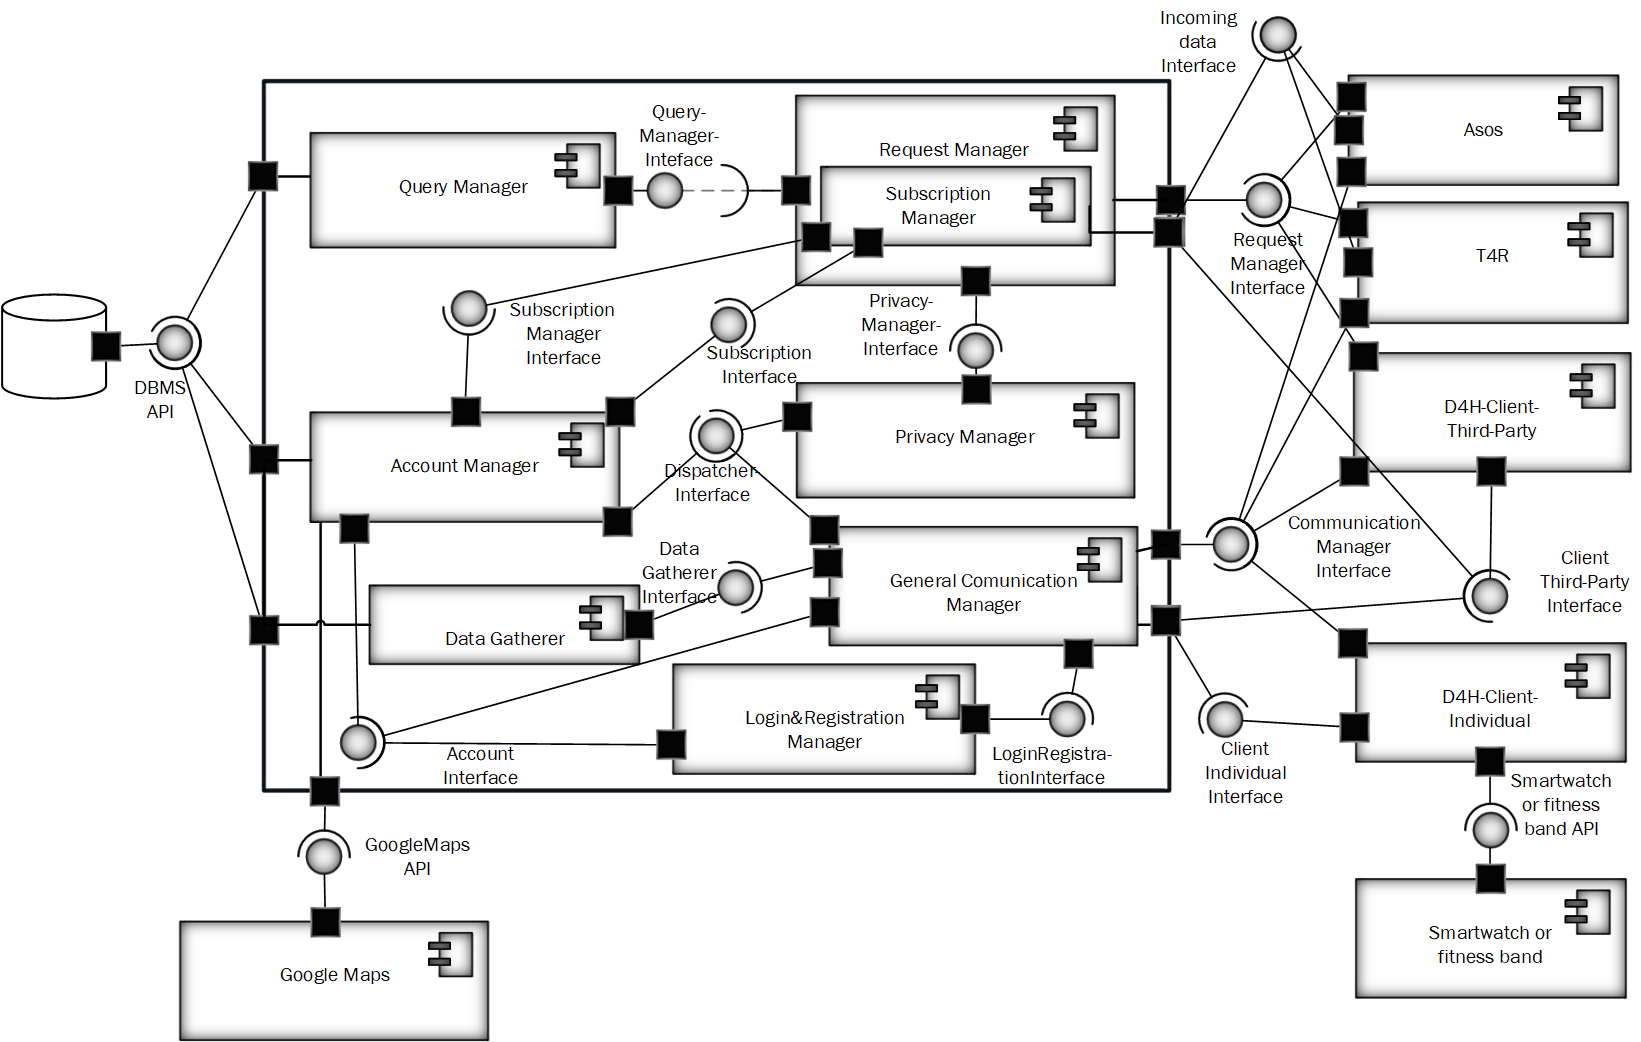
\includegraphics[scale=0.50]{pictures/D4H_componentDiagram.png}}
    \caption{UML Component Diagram of Data4Help system}
    \label{fig:D4H-component}
\end{figure}

Data4Help components are:

\begin{itemize}
    \item \textbf{Login\&registration Manager}:  through \emph{Account Manager}  component, it permits unregistered users to create a new account (either Individual or Third-party) and to already registered users to access their personal profile.
    \item \textbf{Account Manager}: this component allows D4H to manage user accounts; it has to store all the data related to user accounts in the DBMS and show stored data in case of personal data requests. Moreover it needs to communicate with the \emph{Subscription Manager} to store subscription data.
    \item \textbf{Privacy Manager}: it is the component in charge of managing user privacy settings, in particular it asks Individuals for consent during an Individual request (and eventual subscription).
    \item \textbf{Request Manager}: it receives all the request. In case of request without subscription (either Individual or group request) it, itself, handles the request (by querying the db with \emph{Query manager}); if it's a request with subscription, instead, this component forwards the request to its sub-component \emph{Subscription Manager}.
    \item \textbf{Subscription Manager}: it is the component in charge of managing requests with subscription; at the beginning a \emph{Supervisor} object is created; it instantiates a \emph{Worker} at each received request. Periodically the supervisor pings workers and, if someone does not answer, through the \emph{Account Manager} it finds out which subscriptions are lost and creates new workers to substitute them. 
    \item \textbf{Query Manager}: when a request from \emph{Request Manager} arrives, it performs a QUERY to the DBMS.
    \item \textbf{General Communication Manager}: this component acts as a message ``switch" between internal components and external users and viceversa.
    \item \textbf{DBMS}: this is the component for the Database, here D4H stores account data, user gathered data and keeps track of all kinds of requests (single and multiple user, with or without subscription).
    \item \textbf{D4H-Client-Third-party}: this is the Front end for the Third-party client; this component interacts with \emph{General Communication Manager} and \emph{Request Manager}.
    \item \textbf{D4H-Client-Individual}: this is the Front end for the Individual client; this component interacts with the \emph{General Communication Manager}.
    \item \textbf{Smartwatch} or \textbf{Fitness band}: this component represents the external device that D4H system exploits in order to gather Individual data.
    \item \textbf{Google Maps}: this is an external components that D4H uses to map user position on a map.
\end{itemize}


\subsection{AutomatedSOS}

The \textbf{picture \ref{fig:ASOS-component}} is a representation of the UML Component Diagram of AutomatedSOS system. Each component has a specific role in the system and it is better described below. 

\begin{figure}[H]
    \centering
    \makebox[\textwidth][c]{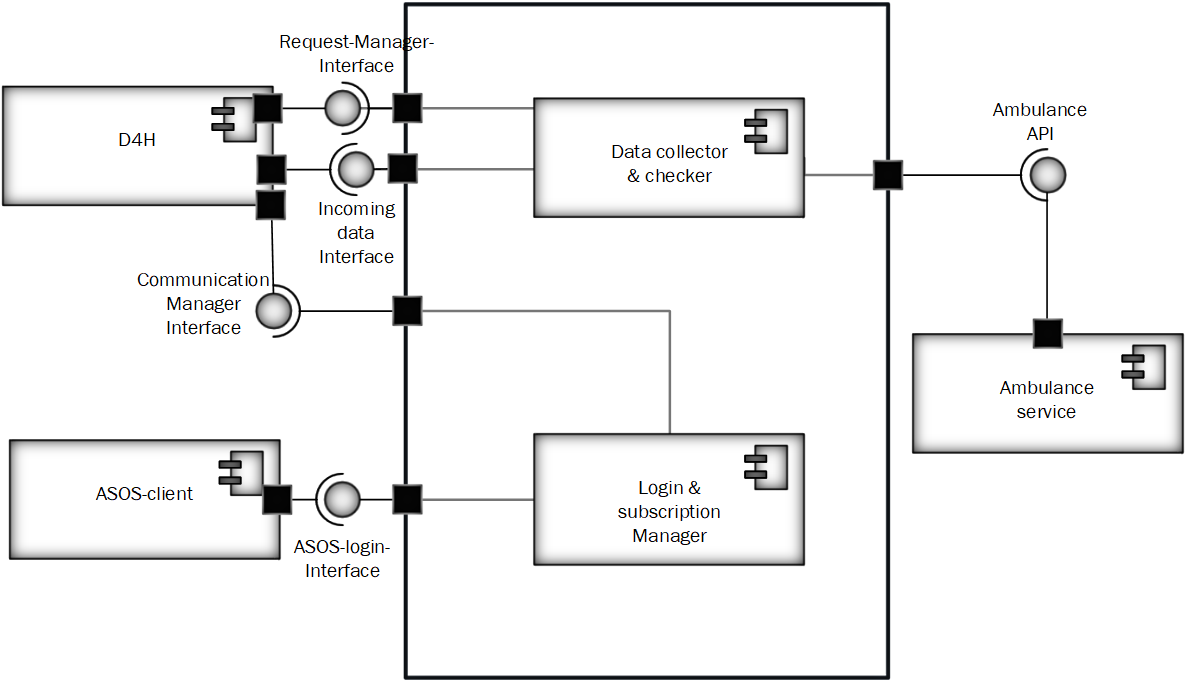
\includegraphics[scale=0.60]{pictures/ASOS-componentDiagram.png}}
    \caption{UML Component Diagram of AutomatedSOS system}
    \label{fig:ASOS-component}
\end{figure}

AutomatedSOS components are:
\begin{itemize}
    \item \textbf{Login\&Registration Manager}: this component allows to sign in using D4H credential, checked through D4H as external component, and to perform a subscription request.
    \item \textbf{Data collector \& Checker}: after a subscription, AutomatedSOS system is ``subscribed in D4H" to the user data and this component receives periodically user gathered data, checks their value and, in case of emergency, dispatches an ambulance, called through the \emph{Ambulance service} component.
    \item \textbf{ASOS-Client}: this is the Front end for the ASOS client; it only interacts with the \emph{Login\&Registration Manager} in order to login and perform a subscription.
    \item \textbf{Ambulance service}: This is the external component representing the Ambulance service that ASOS exploits in order to offer its SOS service.
    \item \textbf{D4H}: this is the external component representing the entire D4H system; ASOS interacts with it using \emph{Communication Manager Interface} to receive gathered data and \emph{Request Manager Interface} to perform subscriptions.
\end{itemize}

\subsection{Track4Run}

The UML Component Diagram for Track4Run is shown in the \textbf{figure \ref{fig:T4R-component}}; the roles that each component plays is defined below.

\begin{figure}[H]
    \centering
    \makebox[\textwidth][c]{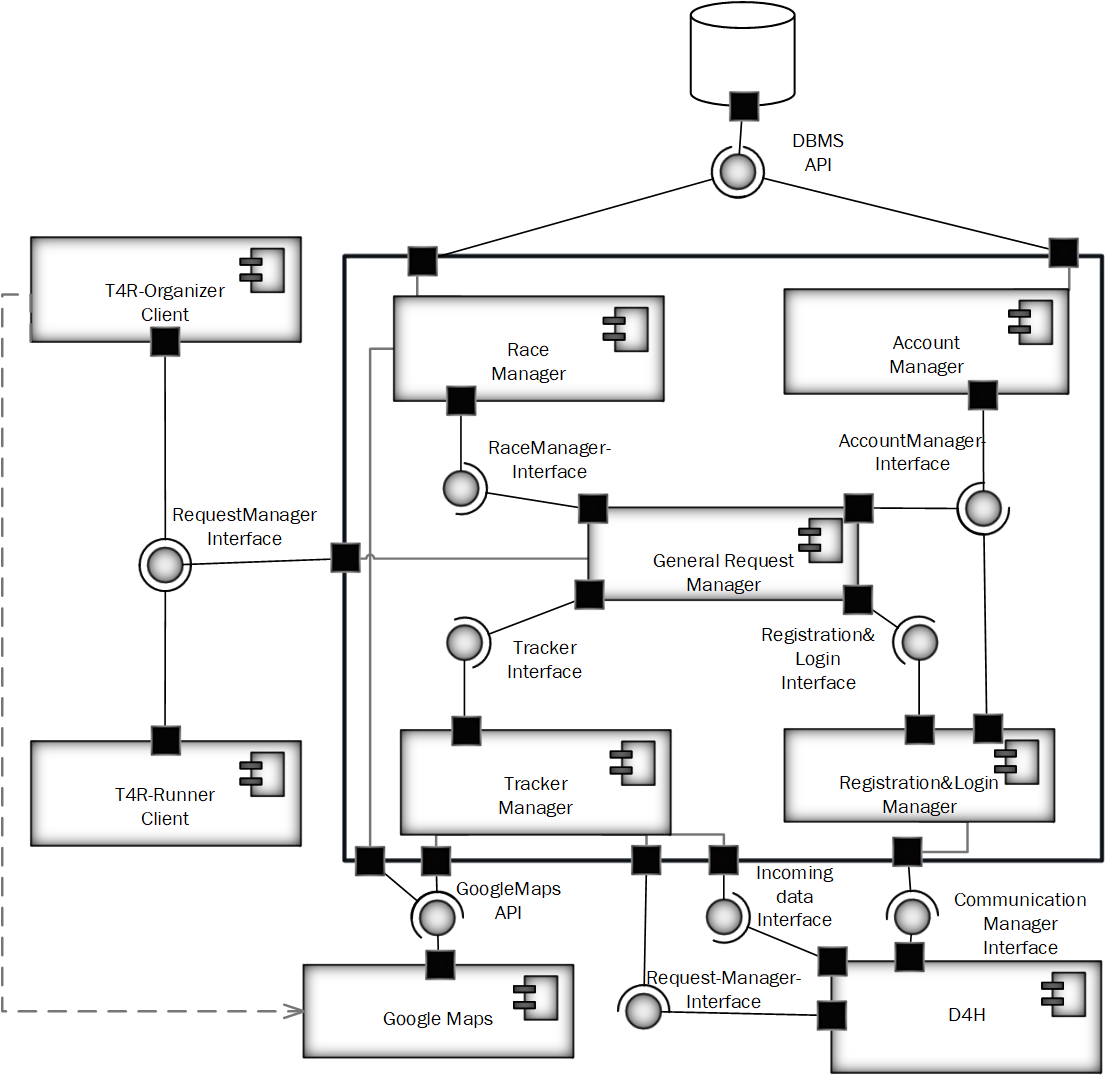
\includegraphics[scale=0.60]{pictures/T4R-componentDiagram.png}}
    \caption{UML Component Diagram of Track4Run system}
    \label{fig:T4R-component}
\end{figure}

Track4Run components are:
\begin{itemize}
    \item \textbf{Registration\&Login Manager}: through the \emph{Account Manager}  component, it permits unregistered users to create a new Organiser account and to already registered users to sign in as Organisers or as Runners using their D4H credentials, checked through D4H as external component.
    \item \textbf{Account Manager}: this component allows T4R to manage user accounts; it has to store all the data related to user accounts in the DBMS, all the data related to races and to show stored data in case of personal data requests.
    \item \textbf{General Request Manager}: this component acts as a message ``switch" between internal components and external users and viceversa.
    \item \textbf{Race Manager}: this is the component in charge of races' management. It creates new runs when a creation request arrives and stores all the data related to races in the DBMS;
    \item \textbf{Tracker Manager}: this component is dedicated to participant tracking; it periodically receives the runners' positions from Data4Help through \emph{Incoming Data Interface}, sends them to \emph{Google Maps}'s external component and forwards computed maps to users (both registered and visitors) that have made requests.
    \item \textbf{T4R-Organizer Client}: this is the Front end for the T4R organiser client; it interacts with the \emph{Race Manager} component to create a new race and with the \emph{Account Manager} component to check the races associated with the Organiser.
    \item \textbf{T4R-Runner Client}: This is the Front end for the T4R participant client; it can make enrolling requests trough the \emph{Race Manager} or ask for its personal data to the \emph{Account Manager} component.
    \item \textbf{D4H}: this is the external component representing the entire D4H system; T4H needs to interact with this component in order to verify Participants credentials and receive the runners' position during a race.
    \item \textbf{Google Maps}: this is an external component that T4R uses to locate runners' positions on a map.
    \item \textbf{DBMS}: this is the component for the Database, here T4R stores users and races data.
\end{itemize}